\documentclass[nobib]{tufte-handout}

\title{Exercise session 5: MSTs, flows, Hamilton cycles and independent sets $\cdot$ 1MA020}

\author[Vilhelm Agdur]{Vilhelm Agdur\thanks{\href{mailto:vilhelm.agdur@math.uu.se}{\nolinkurl{vilhelm.agdur@math.uu.se}}}}

\date{6 November 2023}


%\geometry{showframe} % display margins for debugging page layout

\usepackage{graphicx} % allow embedded images
  \setkeys{Gin}{width=\linewidth,totalheight=\textheight,keepaspectratio}
  \graphicspath{{graphics/}} % set of paths to search for images
\usepackage{amsmath}  % extended mathematics
\usepackage{booktabs} % book-quality tables
\usepackage{units}    % non-stacked fractions and better unit spacing
\usepackage{multicol} % multiple column layout facilities
\usepackage{lipsum}   % filler text
\usepackage{fancyvrb} % extended verbatim environments
  \fvset{fontsize=\normalsize}% default font size for fancy-verbatim environments

\usepackage{color,soul} % Highlights for text

% Standardize command font styles and environments
\newcommand{\doccmd}[1]{\texttt{\textbackslash#1}}% command name -- adds backslash automatically
\newcommand{\docopt}[1]{\ensuremath{\langle}\textrm{\textit{#1}}\ensuremath{\rangle}}% optional command argument
\newcommand{\docarg}[1]{\textrm{\textit{#1}}}% (required) command argument
\newcommand{\docenv}[1]{\textsf{#1}}% environment name
\newcommand{\docpkg}[1]{\texttt{#1}}% package name
\newcommand{\doccls}[1]{\texttt{#1}}% document class name
\newcommand{\docclsopt}[1]{\texttt{#1}}% document class option name
\newenvironment{docspec}{\begin{quote}\noindent}{\end{quote}}% command specification environment

\include{mathcommands.extratex}

\begin{document}

\maketitle% this prints the handout title, author, and date

\begin{abstract}
\noindent
In the previous lecture, we learned how to count the number of spanning trees of a graph. Now, we study how to find spanning trees, and minimal spanning trees. We also think about the vertex version of Eulerian circuits, which are called Hamilton paths. Finally, we consider flows in graphs.
\end{abstract}

\section{Weighted graphs and minimum spanning trees}

We saw in our final theorem of the previous lecture that there is an effective way of computing how many spanning trees there are. Is there also a good way of finding one? The answer to this is yes -- and in fact we can do something much stronger in an efficient way.

To explain the problem we are concerned with, let us introduce the notion of a \emph{weighted} graph. We will consider simple weighted graphs, but the same notion makes perfect sense also for multigraphs and directed graphs.

\begin{definition}
    A \emph{weighted graph} is a simple graph $G = (V,E)$ together with a \emph{weight function} $w: E \to \R$. If $H = (V', E')$ is a subgraph of $G$, its \emph{weight} is defined as $w(H) = \sum_{e\in E'} w(e)$, whenever this is well defined.\sidenote[][-1cm]{If it contains infinitely many positive and infinitely many negative weights, the sum might not converge, but this case is entirely pathological and won't occur for us.} A \emph{minimum spanning tree} (MST) is a spanning tree $T$ of $G$ such that $w(T)$ is minimal among all spanning trees.
\end{definition}

It is clear that for finite weighted graphs, there always exists at least one minimum spanning tree, but they are not necessarily unique -- if all edges have the same weight, then of course every spanning tree is minimal. However, if all edges are given different weights, then the minimum spanning tree is indeed unique.

\begin{xca}
    The things we do here don't work at all for infinite graphs. To demonstrate this, find an infinite weighted graph without a minimum spanning tree. Can you find one with only positive weights?
\end{xca}

\begin{xca}
    Prove that if all edges have different weights, then the minimum spanning tree is unique.
\end{xca}

So we have seen that for finite directed graphs, there does exist a unique minimal spanning tree. How do we find it?

\begin{xca}
  Come up with a reasonable\sidenote[][]{``Reasonable'' here meaning something like at least not brute force, or in polynomial time. The two algorithms we'll look at in the next lecture, and which I'm fishing for with this exercise, run in time $O\left(\abs{E} + \abs{V}\log\left(\abs{V}\right)\right)$ and $\abs{E}\log\left(\abs{V}\right)$ respectively, if implemented optimally.} method for finding a minimum spanning tree. It might be useful here to consider the result we proved two lectures ago, giving four equivalent statements, where one of them was ``$T$ is a tree''.

  One approach might be to build it up by starting at one vertex and then adding in neighbours, and one might be to build it up one edge at a time, making sure never to create a cycle.

  This exercise is likely one of the harder ones on this sheet, so if you get stuck, move on to the later ones.
\end{xca}

If all the weights on our graph are positive, we can interpret the weights on our graph as being distances between vertices, or time it takes to travel between them.\sidenote[][]{If we have negative weights, this of course makes no sense: We can't have negative distances. It would also make a lot of what we are about to do just not work, as we will see in an exercise.} Then it makes sense to make the following definition:

\begin{definition}
  For a weighted graph $G$ with positive edge-weights, we define the \emph{graph distance} between two vertices $v, v' \in G$ by
  $$d_G(v, v') = \min_{\text{walks }P\text{ from }v\text{ to }v'} \sum_{e \in E(P)} w(e).$$
\end{definition}

\begin{xca}
  There's a reason we require positive edge-weights. What could happen if we allowed negative weights? Find an example of a weighted graph with some negative weights where the distance function isn't well-defined.
\end{xca}

It turns out that this notion of graph distance does indeed turn a graph into a metric space, for those of you who know what that is.

\begin{xca}
  Convince yourselves that the following three properties of $d_G$ hold:
  \begin{enumerate}
    \item For all $v, v' \in V$, we have $d_G(v, v') \geq 0$, and $d_G(v,v') = 0$ if and only if $v = v'$.
    \item We have $d_G(v,v') = d_G(v',v)$ for all $v, v' \in V$.
    \item The triangle inequality holds, that is, for all $v, u, w \in V$,
    $$d_G(v, w) \leq d_G(v, u) + d_G(u, w).$$
  \end{enumerate}
\end{xca}

\begin{xca}
  Can you come up with an algorithm to compute the distance between two vertices?

  If you're feeling ambitious, it is actually possible to efficiently find the distances between a fixed vertex $v_0$ and every other vertex in the graph -- how might you do this?
\end{xca}

\section{Flows}

One situation we might want to model using a graph is the flow of traffic in a road network, or of water in a set of pipes. So we imagine we have a bunch of locations, each of which is a vertex, and a collection of edges denoting roads from one location to another, with weights noting how much traffic the road can handle per hour.

To simplify things slightly, we assume all roads are one-directional, and that all vehicles enter the graph through a single \emph{source} vertex in the graph and travel to a \emph{sink} vertex where they leave the graph. 

\begin{xca}
  Can you turn this intuitive description into a formal mathematical definition of a problem to study?
\end{xca}

\begin{figure}
  \centering
  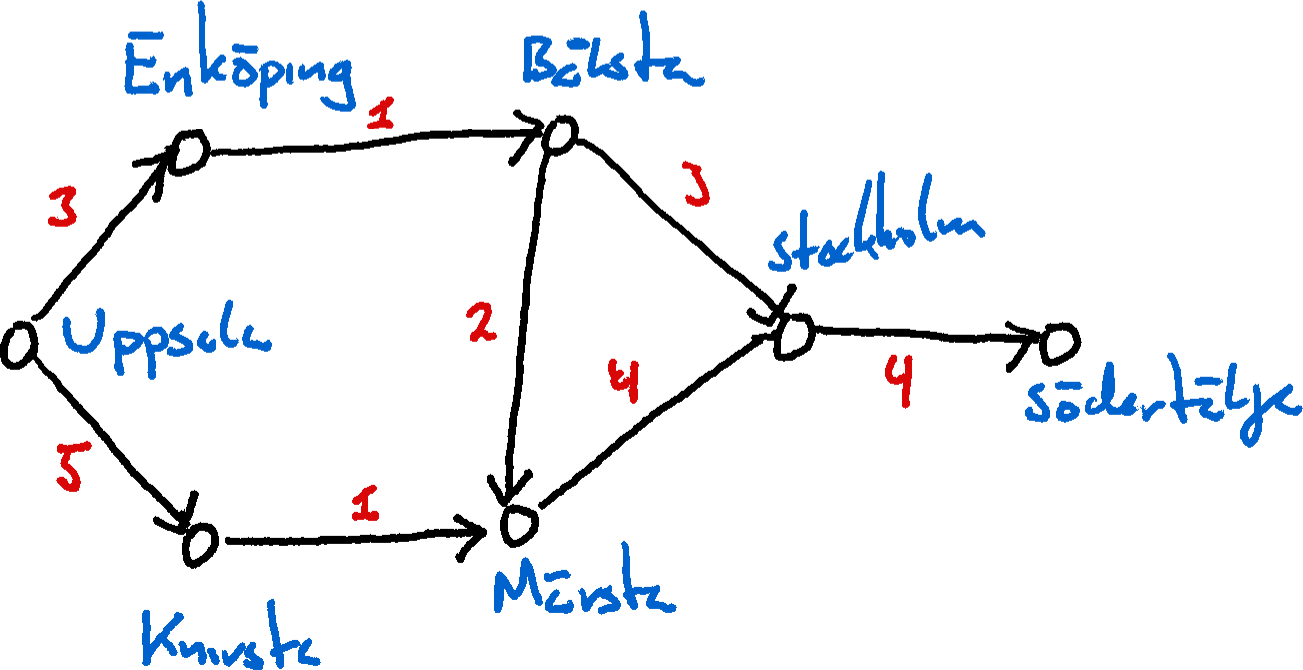
\includegraphics[width=0.85\textwidth]{graphics/L5_exc_MSTs_etc/train_network_flow.png}
  \caption[][0cm]{A hypothetical graph modelling public transport flow from Uppsala to Södertälje.}
  \label{fig:uppsala_stockholm_traffic}
\end{figure}

\begin{xca}
  It should be clear from the intuitive description that we can't have an arbitrary amount of traffic flowing through our graph -- there will always be some upper limit to the traffic, and this will be determined by the worst bottleneck for traffic. 
  
  For example, looking at Figure \ref{fig:uppsala_stockholm_traffic}, it should be obvious that increasing capacity on the Uppsala-Knivsta connection won't improve the flow to Södertälje at all, as long as the Stockholm-Södertälje connection has lower capacity. The only place we can really hope to improve flow as this graph currently looks is by increasing the capacity of either the Enköping-Bålsta or the Knivsta-Märsta connections.
  
  Can you find a rigorous mathematical notion that corresponds to this intuition?
\end{xca}

If you find this interesting or are feeling ambitious, you could even try to figure out an algorithm to determine the maximal flow through the graph. We will give one during the lecture on this.

\section{Hamilton cycles, independent sets, and matchings}

We defined in our first exercise session that a \emph{cycle} in a graph is a walk that starts and ends at the same vertex, but other than that never reuses a vertex. Then we did not use this concept, and instead studied walks that never reuse edges, arriving at the notion of Eulerian circuit.

Now, we will pursue the cycles instead, and define that a \emph{Hamilton cycle} is a cycle that uses every vertex of a graph. We say that a graph is \emph{Hamiltonian} if it has a Hamilton cycle.

\begin{xca}
  For Eulerian circuits there was a rather easy to find method of determining if a graph contains one, and if so of finding one. Is there a similarly easy method to see whether a graph is Hamiltonian?\sidenote[][]{The answer is that there is not -- so the point of the exercise is to just see that the naïve approaches fail.
  
  Or at least, there is no such method assuming $P \neq NP$ -- so if you find one, write it down quick and get that million-dollar Millenium prize.}
\end{xca}

If you are of a more computer-sciencey bent, it may interest you to look up how one proves that determining if a graph is Hamiltonian is NP-complete. It is a fairly neat proof, but not quite simple enough to just give as an exercise.

Another structure that is interesting to study, and where the computational hardness is actually easy to see, is independent sets.

\begin{definition}
  An \emph{independent set} in a graph $G = (V,E)$ is a subset $I$ of the vertices such that no two elements of $I$ are adjacent.
\end{definition}

It turns out that determining if a general graph has an independent set of size $k$ is NP-hard.\sidenote[][]{However, if you restrict to smaller classes of graphs, this may no longer be true -- and there are many results of the form ``if a graph has properties so-and-so, it has an independent set of at least size something'', some of which we might see later in the course.} To show this, let us reduce $3$-SAT to the independent set problem.

\begin{definition}
  A $3$-SAT formula is a formula that looks like
  $$\left(x_1 \vee x_2 \vee \notl x_3\right) \wedge \left(x_2 \vee x_3 \vee \notl x_4\right) \wedge \left(x_1 \vee \notl x_2 \vee x_4\right).$$
  That is, it consists of a conjunction of some number of \emph{clauses}, each of which is a disjunction of three (possibly negated) variables. A \emph{satisfying assignment} is a way to assign the values true or false to each of the variables, so that the entire formula becomes true.\sidenote[][]{This is of course not a real definition -- but it is hopefully clearer about what it actually is than the pile of notation that a real definition would be.}
\end{definition}

\begin{xca}
  We can construct a graph from a $3$-SAT formula as follows: For each clause, draw a triangle, labelling each vertex of the triangle with one of the variables in the disjunction, including whether it was negated or not. Then draw an edge between any two vertices labelled $x_i$ and $\notl x_i$ for every $i$.

  Do this for the $3$-SAT formula we gave in our ``definition''. Show that there is a satistfying assignment for the $3$-SAT formula if and only if there is an independent set of size $k$ in the corresponding graph. This will show that the independent set problem is NP-Hard.
\end{xca}

One final structure we are going to study in a graph is a so-called \emph{matching}.

\begin{definition}
  A \emph{matching} in a graph $G = (V,E)$ is a set of edges $M \subseteq E$ such that no two edges in $M$ share an endpoint. If $\{v, w\} \in M$ we say that $v$ and $w$ have been matched to each other.
\end{definition}

It turns out that this concept is actually closely related to that of independent sets, if you squint at it in the right way.

\begin{definition}
  Given a graph $G = (V, E)$, the \emph{line graph} $L(G)$ of $G$ has as its vertices the \emph{edges} of $G$, and there is an edge between $e$ and $e'$ whenever they share an endpoint in $G$.
\end{definition}

\begin{xca}
  Convince yourselves that a matching in $G$ and an independent set in $L(G)$ are precisely the same thing.
\end{xca}

%\bibliography{references}
%\bibliographystyle{plainnat}

\end{document}
